\documentclass[12pt]{article}
\usepackage[left=1cm, right=1cm, top=2cm,bottom=1.5cm]{geometry} 

\usepackage[parfill]{parskip}
\usepackage[utf8]{inputenc}
\usepackage[T2A]{fontenc}
\usepackage[russian]{babel}
\usepackage{enumitem}
\usepackage[normalem]{ulem}
\usepackage{amsfonts, amsmath, amsthm, amssymb, mathtools,xcolor}
\usepackage{blkarray}

\usepackage{tabularx}
\usepackage{hhline}

\usepackage{accents}
\usepackage{fancyhdr}
\pagestyle{fancy}
\renewcommand{\headrulewidth}{1.5pt}
\renewcommand{\footrulewidth}{1pt}

\usepackage{graphicx}
\usepackage[figurename=Рис.]{caption}
\usepackage{subcaption}
\usepackage{float}

%%Наименование папки откуда забирать изображения
\graphicspath{ {./images/} }

%%Изменение формата для ввода доказательства
\renewcommand{\proofname}{$\square$  \nopunct}
\renewcommand\qedsymbol{$\blacksquare$}

%%Изменение отступа на таблицах
\addto\captionsrussian{%
	\renewcommand{\proofname}{$\square$ \nopunct}%
}
%% Римские цифры
\newcommand{\RN}[1]{%
	\textup{\uppercase\expandafter{\romannumeral#1}}%
}

%% Для удобства записи
\newcommand{\MR}{\mathbb{R}}
\newcommand{\MC}{\mathbb{C}}
\newcommand{\MQ}{\mathbb{Q}}
\newcommand{\MN}{\mathbb{N}}
\newcommand{\MZ}{\mathbb{Z}}
\newcommand{\MTB}{\mathbb{T}}
\newcommand{\MTI}{\mathbb{I}}
\newcommand{\MI}{\mathrm{I}}
\newcommand{\MCI}{\mathcal{I}}
\newcommand{\MJ}{\mathrm{J}}
\newcommand{\MH}{\mathrm{H}}
\newcommand{\MT}{\mathrm{T}}
\newcommand{\MU}{\mathcal{U}}
\newcommand{\MV}{\mathcal{V}}
\newcommand{\MB}{\mathcal{B}}
\newcommand{\MF}{\mathcal{F}}
\newcommand{\MW}{\mathcal{W}}
\newcommand{\ML}{\mathcal{L}}
\newcommand{\MP}{\mathcal{P}}
\newcommand{\VN}{\varnothing}
\newcommand{\VE}{\varepsilon}
\newcommand{\dx}{\, dx}
\newcommand{\dy}{\, dy}
\newcommand{\dz}{\, dz}
\newcommand{\dd}{\, d}


\theoremstyle{definition}
\newtheorem{defn}{Опр:}
\newtheorem{rem}{Rm:}
\newtheorem{prop}{Утв.}
\newtheorem{exrc}{Упр.}
\newtheorem{problem}{Задача}
\newtheorem{lemma}{Лемма}
\newtheorem{theorem}{Теорема}
\newtheorem{corollary}{Следствие}

\newenvironment{cusdefn}[1]
{\renewcommand\thedefn{#1}\defn}
{\enddefn}

\DeclareRobustCommand{\divby}{%
	\mathrel{\text{\vbox{\baselineskip.65ex\lineskiplimit0pt\hbox{.}\hbox{.}\hbox{.}}}}%
}
%Короткий минус
\DeclareMathSymbol{\SMN}{\mathbin}{AMSa}{"39}
%Длинная шапка
\newcommand{\overbar}[1]{\mkern 1.5mu\overline{\mkern-1.5mu#1\mkern-1.5mu}\mkern 1.5mu}
%Функция знака
\DeclareMathOperator{\sgn}{sgn}

%Функция ранга
\DeclareMathOperator{\rk}{\text{rk}}
\DeclareMathOperator{\diam}{\text{diam}}


%Обозначение константы
\DeclareMathOperator{\const}{\text{const}}

\DeclareMathOperator{\codim}{\text{codim}}

\DeclareMathOperator*{\dsum}{\displaystyle\sum}
\newcommand{\ddsum}[2]{\displaystyle\sum\limits_{#1}^{#2}}

%Интеграл в большом формате
\DeclareMathOperator{\dint}{\displaystyle\int}
\newcommand{\ddint}[2]{\displaystyle\int\limits_{#1}^{#2}}
\newcommand{\ssum}[1]{\displaystyle \sum\limits_{n=1}^{\infty}{#1}_n}

\newcommand{\smallerrel}[1]{\mathrel{\mathpalette\smallerrelaux{#1}}}
\newcommand{\smallerrelaux}[2]{\raisebox{.1ex}{\scalebox{.75}{$#1#2$}}}

\newcommand{\smallin}{\smallerrel{\in}}
\newcommand{\smallnotin}{\smallerrel{\notin}}

\newcommand*{\medcap}{\mathbin{\scalebox{1.25}{\ensuremath{\cap}}}}%
\newcommand*{\medcup}{\mathbin{\scalebox{1.25}{\ensuremath{\cup}}}}%

\makeatletter
\newcommand{\vast}{\bBigg@{3.5}}
\newcommand{\Vast}{\bBigg@{5}}
\makeatother

%Промежуточное значение для sup\inf, поскольку они имеют разную высоту
\newcommand{\newsup}{\mathop{\smash{\mathrm{sup}}}}
\newcommand{\newinf}{\mathop{\mathrm{inf}\vphantom{\mathrm{sup}}}}

%Скалярное произведение
\newcommand{\inner}[2]{\left\langle #1, #2 \right\rangle }
\newcommand{\linsp}[1]{\left\langle #1 \right\rangle }
\newcommand{\linmer}[2]{\left\langle #1 \vert #2\right\rangle }

%Подпись символов снизу
\newcommand{\ubar}[1]{\underaccent{\bar}{#1}}

%% Шапка для букв сверху
\newcommand{\wte}[1]{\widetilde{#1}}
\newcommand{\wht}[1]{\widehat{#1}}

%%Трансформация Фурье
\newcommand{\fourt}[1]{\mathcal{F}\left(#1\right)}
\newcommand{\ifourt}[1]{\mathcal{F}^{-1}\left(#1\right)}

%%Символ вектора
\newcommand{\vecm}[1]{\overrightarrow{#1\,}}

%%Пространстов матриц
\newcommand{\mat}[2]{\operatorname{Mat}_{#1\times #2}}

%Оператор для действ и мнимых чисел
\DeclareMathOperator{\IM}{\operatorname{Im}}
\DeclareMathOperator{\RE}{\operatorname{Re}}
\DeclareMathOperator{\li}{\operatorname{li}}


%%Взятие в скобки, модули и норму
\newcommand{\parfit}[1]{\left( #1 \right)}
\newcommand{\modfit}[1]{\left| #1 \right|}
\newcommand{\sqparfit}[1]{\left\{ #1 \right\}}
\newcommand{\normfit}[1]{\left\| #1 \right\|}

%%Функция для обозначения равномерной сходимости по множеству
\newcommand{\uconv}[1]{\overset{#1}{\rightrightarrows}}
\newcommand{\uconvm}[2]{\overset{#1}{\underset{#2}{\rightrightarrows}}}


%%Функция для обозначения нижнего и верхнего интегралов
\def\upint{\mathchoice%
	{\mkern13mu\overline{\vphantom{\intop}\mkern7mu}\mkern-20mu}%
	{\mkern7mu\overline{\vphantom{\intop}\mkern7mu}\mkern-14mu}%
	{\mkern7mu\overline{\vphantom{\intop}\mkern7mu}\mkern-14mu}%
	{\mkern7mu\overline{\vphantom{\intop}\mkern7mu}\mkern-14mu}%
	\int}
\def\lowint{\mkern3mu\underline{\vphantom{\intop}\mkern7mu}\mkern-10mu\int}

%%След матрицы
\DeclareMathOperator*{\tr}{tr}

\makeatletter
\renewcommand*\env@matrix[1][*\c@MaxMatrixCols c]{%
	\hskip -\arraycolsep
	\let\@ifnextchar\new@ifnextchar
	\array{#1}}
\makeatother


%% Переопределение функции хи, чтобы выглядела более приятно
\makeatletter
\@ifdefinable\@latex@chi{\let\@latex@chi\chi}
\renewcommand*\chi{{\@latex@chi\smash[t]{\mathstrut}}} % want only bottom half of \mathstrut
\makeatletter

\begin{document}
\lhead{Математический анализ - \RN{2}}
\chead{Косухин О.Н.}
\rhead{Семинар - 8}

\section*{Определенный интеграл}
Начнем с интеграла Римана. Пусть есть отрезок $[a,b]$ и какая-то функция $f(x)$ (пусть пока непрерывная). Мы хотим определить понятие площади подграфика функции.
\begin{defn}
	\uwave{Подграфик функции} - фигура заключенная между графиком функции и осью $Ox$. Если график выше оси $Ox$ - то будем считать её со знаком $+$, если ниже, то со знаком $-$.
\end{defn}
\textbf{Подход Римана}: порежем отрезок $[a,b]$ на части другими отрезками - зададим набор точек:
$$
	a = x_0 < x_1 < x_2 < \dotsc < x_{n-1} < b = x_n
$$
То есть, мы задали разбинеие отрезка и хотим приблизить площадь подграфика прямоугольниками и задали их горизонтальные стороны, но пока не хватает высоты. Возникает вопрос на какой высоте её проводить, чтобы это было разумно? 

Разумно было бы выбрать какую-то точку $\xi_j$ на отрезках $[x_{j-1},x_j]$ и высоту планки задать значением функции в этой точке. Разбиение обычно обозначают как $\MTB$, набор отмеченных точек как $\{\xi_j\}$.

\begin{figure}[H]
	\centering
	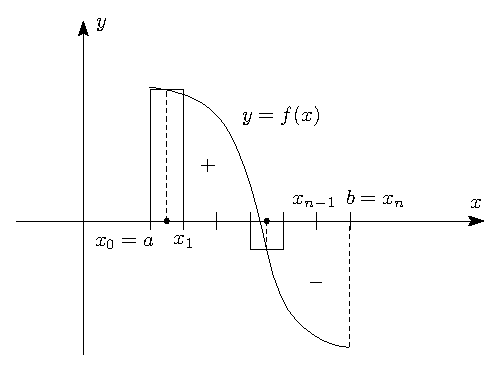
\includegraphics[width=0.45\textwidth]{MA2S8_1.eps}
	\caption{Поиск площади подграфика функции $f(x)$.}
	\label{8_1}
\end{figure}

Таким образом, у нас получается некая ``подмена'' площади в виде суммы площадей прямоугольников, которые образуются на графике функции:
$$
	\sigma(f,\MTB,\xi) = \ddsum{j = 1}{n}f(\xi_j){\cdot}(x_j - x_{j-1})
$$
\begin{defn}
	\uwave{База} $\MB$ это набор множеств таких, что:
	\begin{enumerate}[label=\arabic*)]
		\item $B \in \MB \Rightarrow B \neq \VN$;
		\item $B_1,B_2 \in \MB \Rightarrow B_1 \cap B_2 \neq \VN, \, \exists \, B_3 \colon B_3 \subset B_1 \cap B_2$;
	\end{enumerate}
\end{defn}
На лекциях проходили, что предел по базе обладает теми привичными свойствами, которые обсуждали для пределов последовательностей и функций.

Мы задаем базу на разбиениях $\MTB$ и вводим понятие $\lambda(\MTB)$ - диаметр $\MTB$:
$$
	\lambda(\MTB) = \max\limits_{j}|x_j - x_{j-1}|
$$
Тогда у нас появляются элементы базы:
$$
	B_\VE = \{\MTB \colon \lambda{(\MTB)} < \VE\}
$$
Понятно, что можно придумать какое-то разбиение, которое будет меньше наперед заданного $\VE > 0$. Понятно, что с уменьшением $\VE$ множество $B_{\VE}$ тоже уменьшается, но остается непустым $\Rightarrow$ множество таких $B_{\VE}$ является базой. Следовательно, можно рассматривать предел по базе:
$$
	\lim\limits_{\lambda(\MTB) \to 0} \sigma(f,\MTB,\xi) = \MI
$$
Бросается в глаза то, что накладывается ограничение на $\xi_j$: требуется $\xi_j \in [x_{j} - x_{j-1}] = \Delta_j$. При этом эти $\xi_j$ не фигурируют в определениях для $B_\VE$ и для $\MI$. Оказывается, не для всех функций мы можем посчитать такой интеграл. Если мы уже выбрали разбиение $\MTB$, какова свобода для интегральной суммы? В каких пределах она может меняться?
\begin{figure}[H]
	\centering
	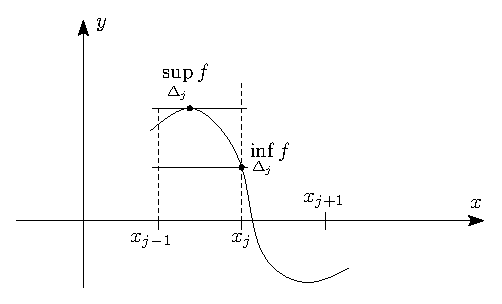
\includegraphics[width=0.55\textwidth]{MA2S8_2.eps}
	\caption{Верхняя и нижняя сумма Дарбу для $f(x)$.}
	\label{8_2}
\end{figure}
На отрезке $\Delta_j$ планку, которую мы можем провести колеблется от $\inf\limits_{\Delta_j}f(x)$ до $\sup\limits_{\Delta_j}f(x)$. Таким образом, интегральная сумма колеблется между нижней и верхней суммой Дарбу:
\begin{defn}
	\uwave{Нижняя сумма Дарбу}:
	$$
		s(f,\MTB) = \ddsum{j = 1}{n}\inf\limits_{\Delta_j}f{\cdot}\Delta_j
	$$
\end{defn}
\begin{defn}
	\uwave{Верхняя сумма Дарбу}:
	$$
		S(f,\MTB) =  \ddsum{j = 1}{n}\sup\limits_{\Delta_j}f{\cdot}\Delta_j
	$$
\end{defn}

Всегда выполняется неравенство:
$$
	S(f,\MTB) \geq \sigma(f,\MTB,\xi) \geq s(f,\MTB)
$$
Если мы будем брать разные разбиения $\MTB$ и будем отмечать на действительной прямой значения верхней и нижней суммы Дарбу, то они будут образовывать множества, которые отделены друг от друга:
\begin{figure}[H]
	\centering
	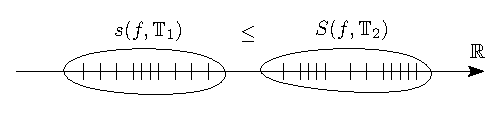
\includegraphics[width=0.45\textwidth]{MA2S8_3.eps}
	\caption{Отделение множеств верхних и нижних сумм Дарбу для разных разбиений $\MTB_1$ и $\MTB_2$.}
	\label{8_3}
\end{figure}
Оказывается, что функцию мы можем проинтегрировать тогда и только тогда, когда такие множества соприкасаются по точке, которая и будет являться искомым интегралом:
$$
	\inf\limits_{\MTB}S(f,\MTB) = \sup\limits_{\MTB}s(f,\MTB) = \ddint{a}{b}f(x)dx
$$
\begin{figure}[H]
	\centering
	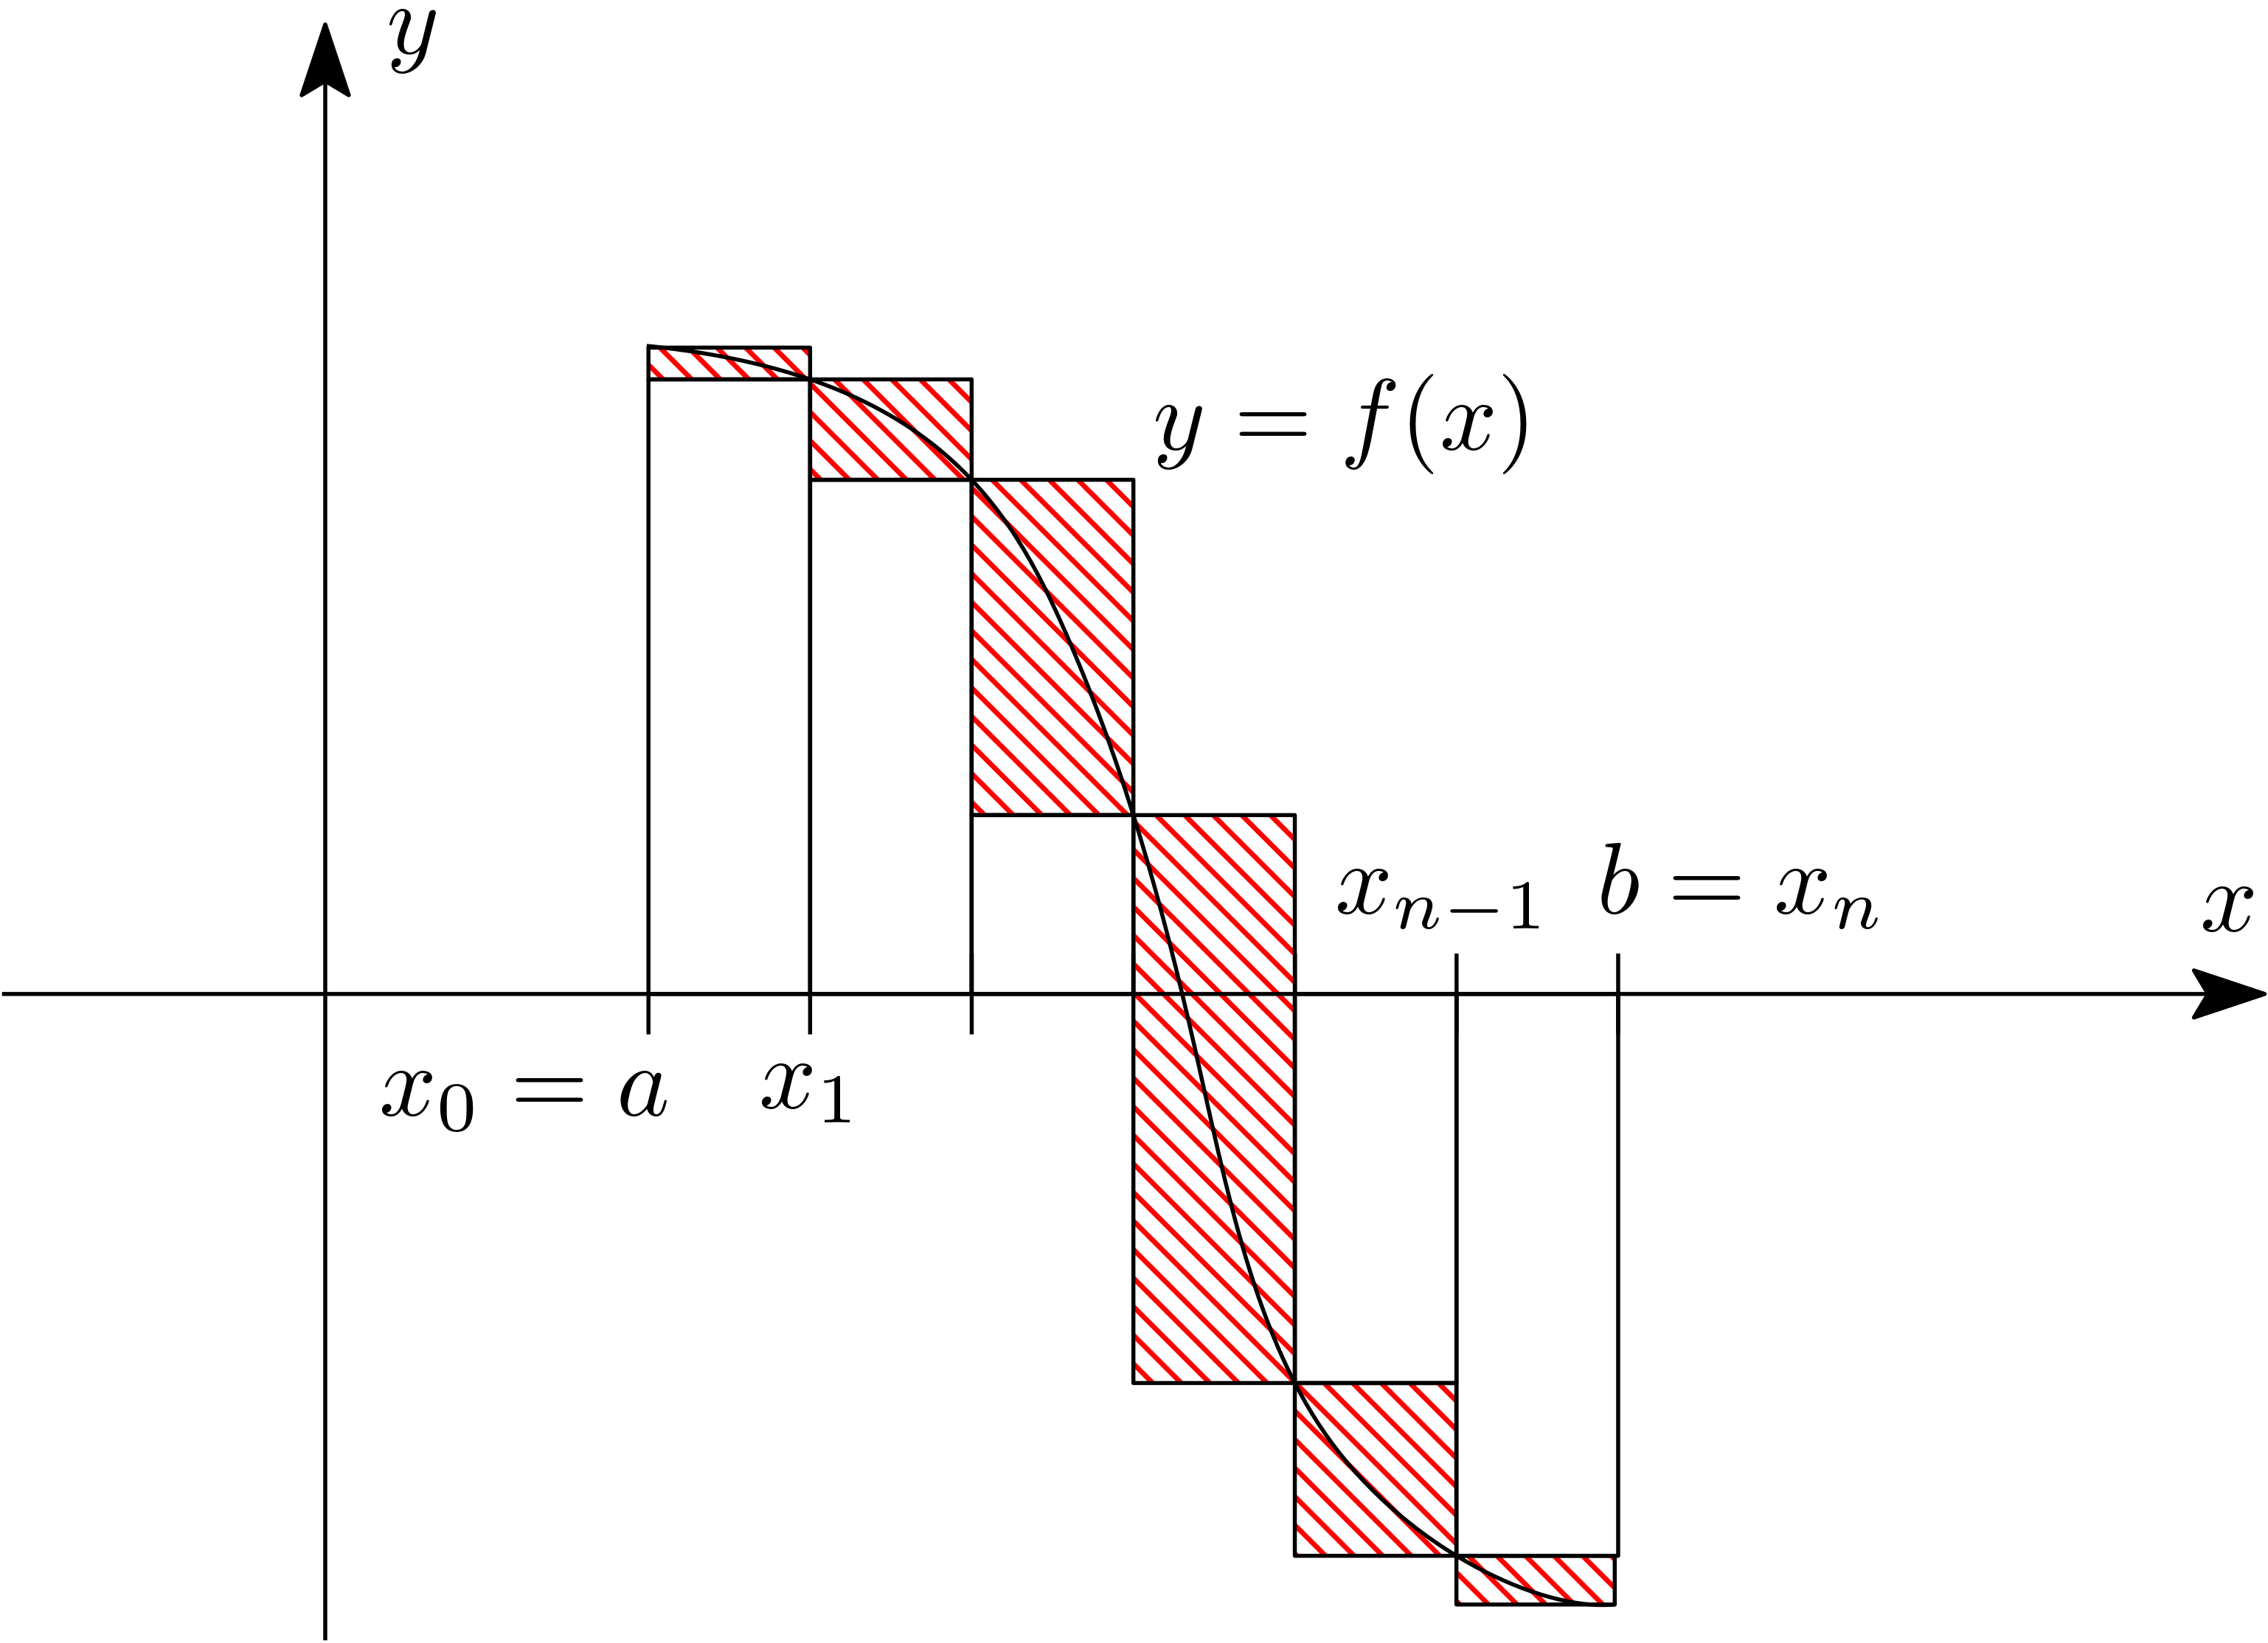
\includegraphics[width=0.45\textwidth]{MA2S8_4.png}
	\caption{Зазор между верхними и нижними суммами Дарбу.}
	\label{8_4}
\end{figure}
\begin{defn}
	\uwave{Колебания функции} на отрезке разбиения $\Delta_j$:
	$$
		\omega_j = \sup\limits_{\Delta_j}f - \inf\limits_{\Delta_j}f
	$$
\end{defn}
\begin{defn}
	\uwave{Омега-сумма} это сумма колебаний функций, умноженных на длину отрезка:
	$$
		\Omega(\MTB) = \ddsum{j=1}{n}\omega_j(\MTB){\cdot}\Delta_j = S(\MTB) - s(\MTB)
	$$
\end{defn}

\textbf{Критерий интегрируемости Дарбу}:
$$
	\exists \, \lim\limits_{\lambda(\MTB) \to 0}\sigma(f,\MTB,\xi) = \MI = \ddint{a}{b}f(x)dx \Leftrightarrow \forall \VE > 0, \, \exists \, \MTB \colon \Omega(\MTB) < \VE
$$
В частности отсюда следует, что интегрируемыми по Риману являются непрерывные функции, ограниченные функции у которых конечно количество точек разрыва или монотонные функции. Если же функций неограничена, то она не интегрируема по Риману (если функция неограничена $\Rightarrow$ неограничена на каком-то отрезке $\Rightarrow$ не сможем покрыть прямоугольником конечной площади этот график $\Rightarrow$ омега-сумма будет больше $\VE$.)
\newpage
Рассмотрим ограниченную функцию у которой очень много точек разрыва:
\begin{problem}(\textbf{Д2197})
	Рассмотрим функцию Дирихле:
	$$
		\chi(x) = 
		\begin{cases}
			1, & x \in \MQ \\
			0, & x \in \MR \setminus \MQ
		\end{cases}
	$$
\end{problem}
\begin{proof}
	Как бы мы ни резали отрезок $[a,b]$ на части у нас в любом маленьком отрезке есть как рациональная точка, так и иррациональная точка, поэтому:
	$$
		\forall j = \overline{1,n}, \, \sup\limits_{\Delta_j}\chi = 1, \, \inf\limits_{\Delta_j}\chi = 0 \Rightarrow \Omega(\MTB) = (b-a){\cdot}1 > 0
	$$
	Таким образом, эта функция не интегрируема.
\end{proof}

\begin{problem}(\textbf{Д2182 а)})
	Написать верхнюю и нижнюю интегральные суммы для $f(x) = x^3$ на отрезке $[-2,3]$ с разбиением на $n$ равных частей.
\end{problem}
\begin{proof}
	Берем отрезок $[-2,3]$, выбираем некоторое натуральное $n$ и делим этот отрезок на $n$ равных частей, каждый длины: $\tfrac{3 -  (-2)}{n} = \tfrac{5}{n}$, отмеченные точки выглядят следующим образом:
	$$
		x_0 = -2,  x_1 = -2 + \dfrac{5}{n}, \dotsc, x_j = -2 + \dfrac{5}{n}j, \dotsc, x_n = 3 \Rightarrow \lambda(\MTB) = \dfrac{5}{n}
	$$
	Посчитаем суммы Дарбу:
	$$
		S(f,\MTB) = f(x_1){\cdot}\dfrac{5}{n} + f(x_2){\cdot}\dfrac{5}{n} + \dotsc + f(x_n){\cdot}\dfrac{5}{n}
	$$
	$$
		s(f,\MTB) = f(x_0){\cdot}\dfrac{5}{n} + f(x_1){\cdot}\dfrac{5}{n} + \dotsc + f(x_{n-1}){\cdot}\dfrac{5}{n}
	$$
	$$
		\Omega(\MTB) = S(f,\MTB)- s(f,\MTB) = (f(x_n) - f(x_0)){\cdot}\dfrac{5}{n} = (f(b) - f(a)){\cdot}\dfrac{5}{n} \to 0
	$$
	Таким образом, верхняя и нижняя суммы Дарбу смыкаются друг с другом $\Rightarrow$ для любого $\VE > 0$ можно подобрать верхнюю/нижнюю сумму, которые будут отличатсья меньше, чем на $\VE \Rightarrow$ функция интегрируема. Мы даже сможем посчитать интеграл, поскольку к нему будет стремиться как нижняя сумма Дарбу, так и верхняя (в данном случае они будут также интегральными суммами). Рассмотрим к примеру нижнюю сумму:
	$$
		s(f,\MTB) = \dfrac{5}{n}{\cdot}\left((-2)^3 + \left( -2 + \dfrac{5}{n}\right)^3 + \dotsc + \left( -2 + \dfrac{5(n-1)}{n}\right)^3 \right) = 
	$$
	$$
		=\dfrac{5}{n}{\cdot}\left((-2)^3{\cdot}n + 3{\cdot}(-2)^2{\cdot}\left(\dfrac{5}{n} + 2{\cdot}\dfrac{5}{n} + \dotsc + (n-1){\cdot}\dfrac{5}{n} \right) + 3{\cdot}(-2){\cdot}\left( \left(\dfrac{5}{n}\right)^2  + \dotsc + \left((n-1){\cdot}\dfrac{5}{n}\right)^2\right) + \dotsc\right)
	$$
	где справа - сумма кубов. Поскольку мы знаем:
	$$
		1^2 + \dotsc + k^2 = \dfrac{k(k+1)(2k+1)}{6}, \, 1^3 + \dotsc + k^3 = \left(\dfrac{k(k+1)}{2}\right)^2
	$$
	то мы можем в явном виде посчитать интеграл, воспользовавшись формулами выше и найдя отношение двух  многочленов $\Rightarrow$ можно будет найти его предел.
\end{proof}

\begin{problem}(\textbf{Д2193.1})
	$f(x)$ - монотонна на $[0,1]$, тогда:
	$$
		\ddint{0}{1}f(x)dx - \dfrac{1}{n}\ddsum{k = 1}{n}f\left(\dfrac{k}{n}\right) = O\left(\dfrac{1}{n}\right)
	$$
\end{problem}
\begin{proof}
	Пусть $f(x)$ - неубывающая. Поделим отрезок $[0,1]$ на $n$ равных частей.
	\begin{figure}[H]
		\centering
		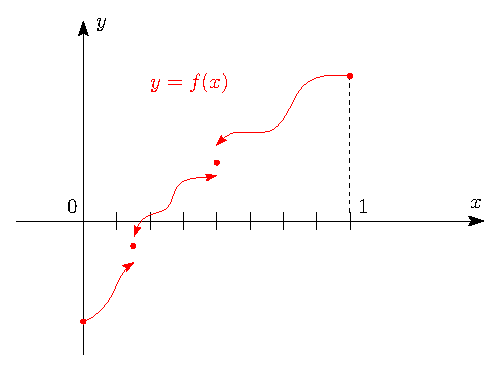
\includegraphics[width=0.45\textwidth]{MA2S8_5.eps}
		\caption{Монотонная неубывающая функция $f(x)$ на $[0,1]$.}
		\label{8_5}
	\end{figure}
	То, что мы вычитаем из функции на самом деле это верхняя сумма Дарбу:
	$$
		S(f,\MTB) = \dfrac{1}{n}\ddsum{k = 1}{n}f\left(\dfrac{k}{n}\right)
	$$
	Это так, поскольку супремум монотонно неубывающей функции совпадает со значением в крайней правой точке на отрезке. Построим зазор между верхней и нижней суммой Дарбу.
	\begin{figure}[H]
		\centering
		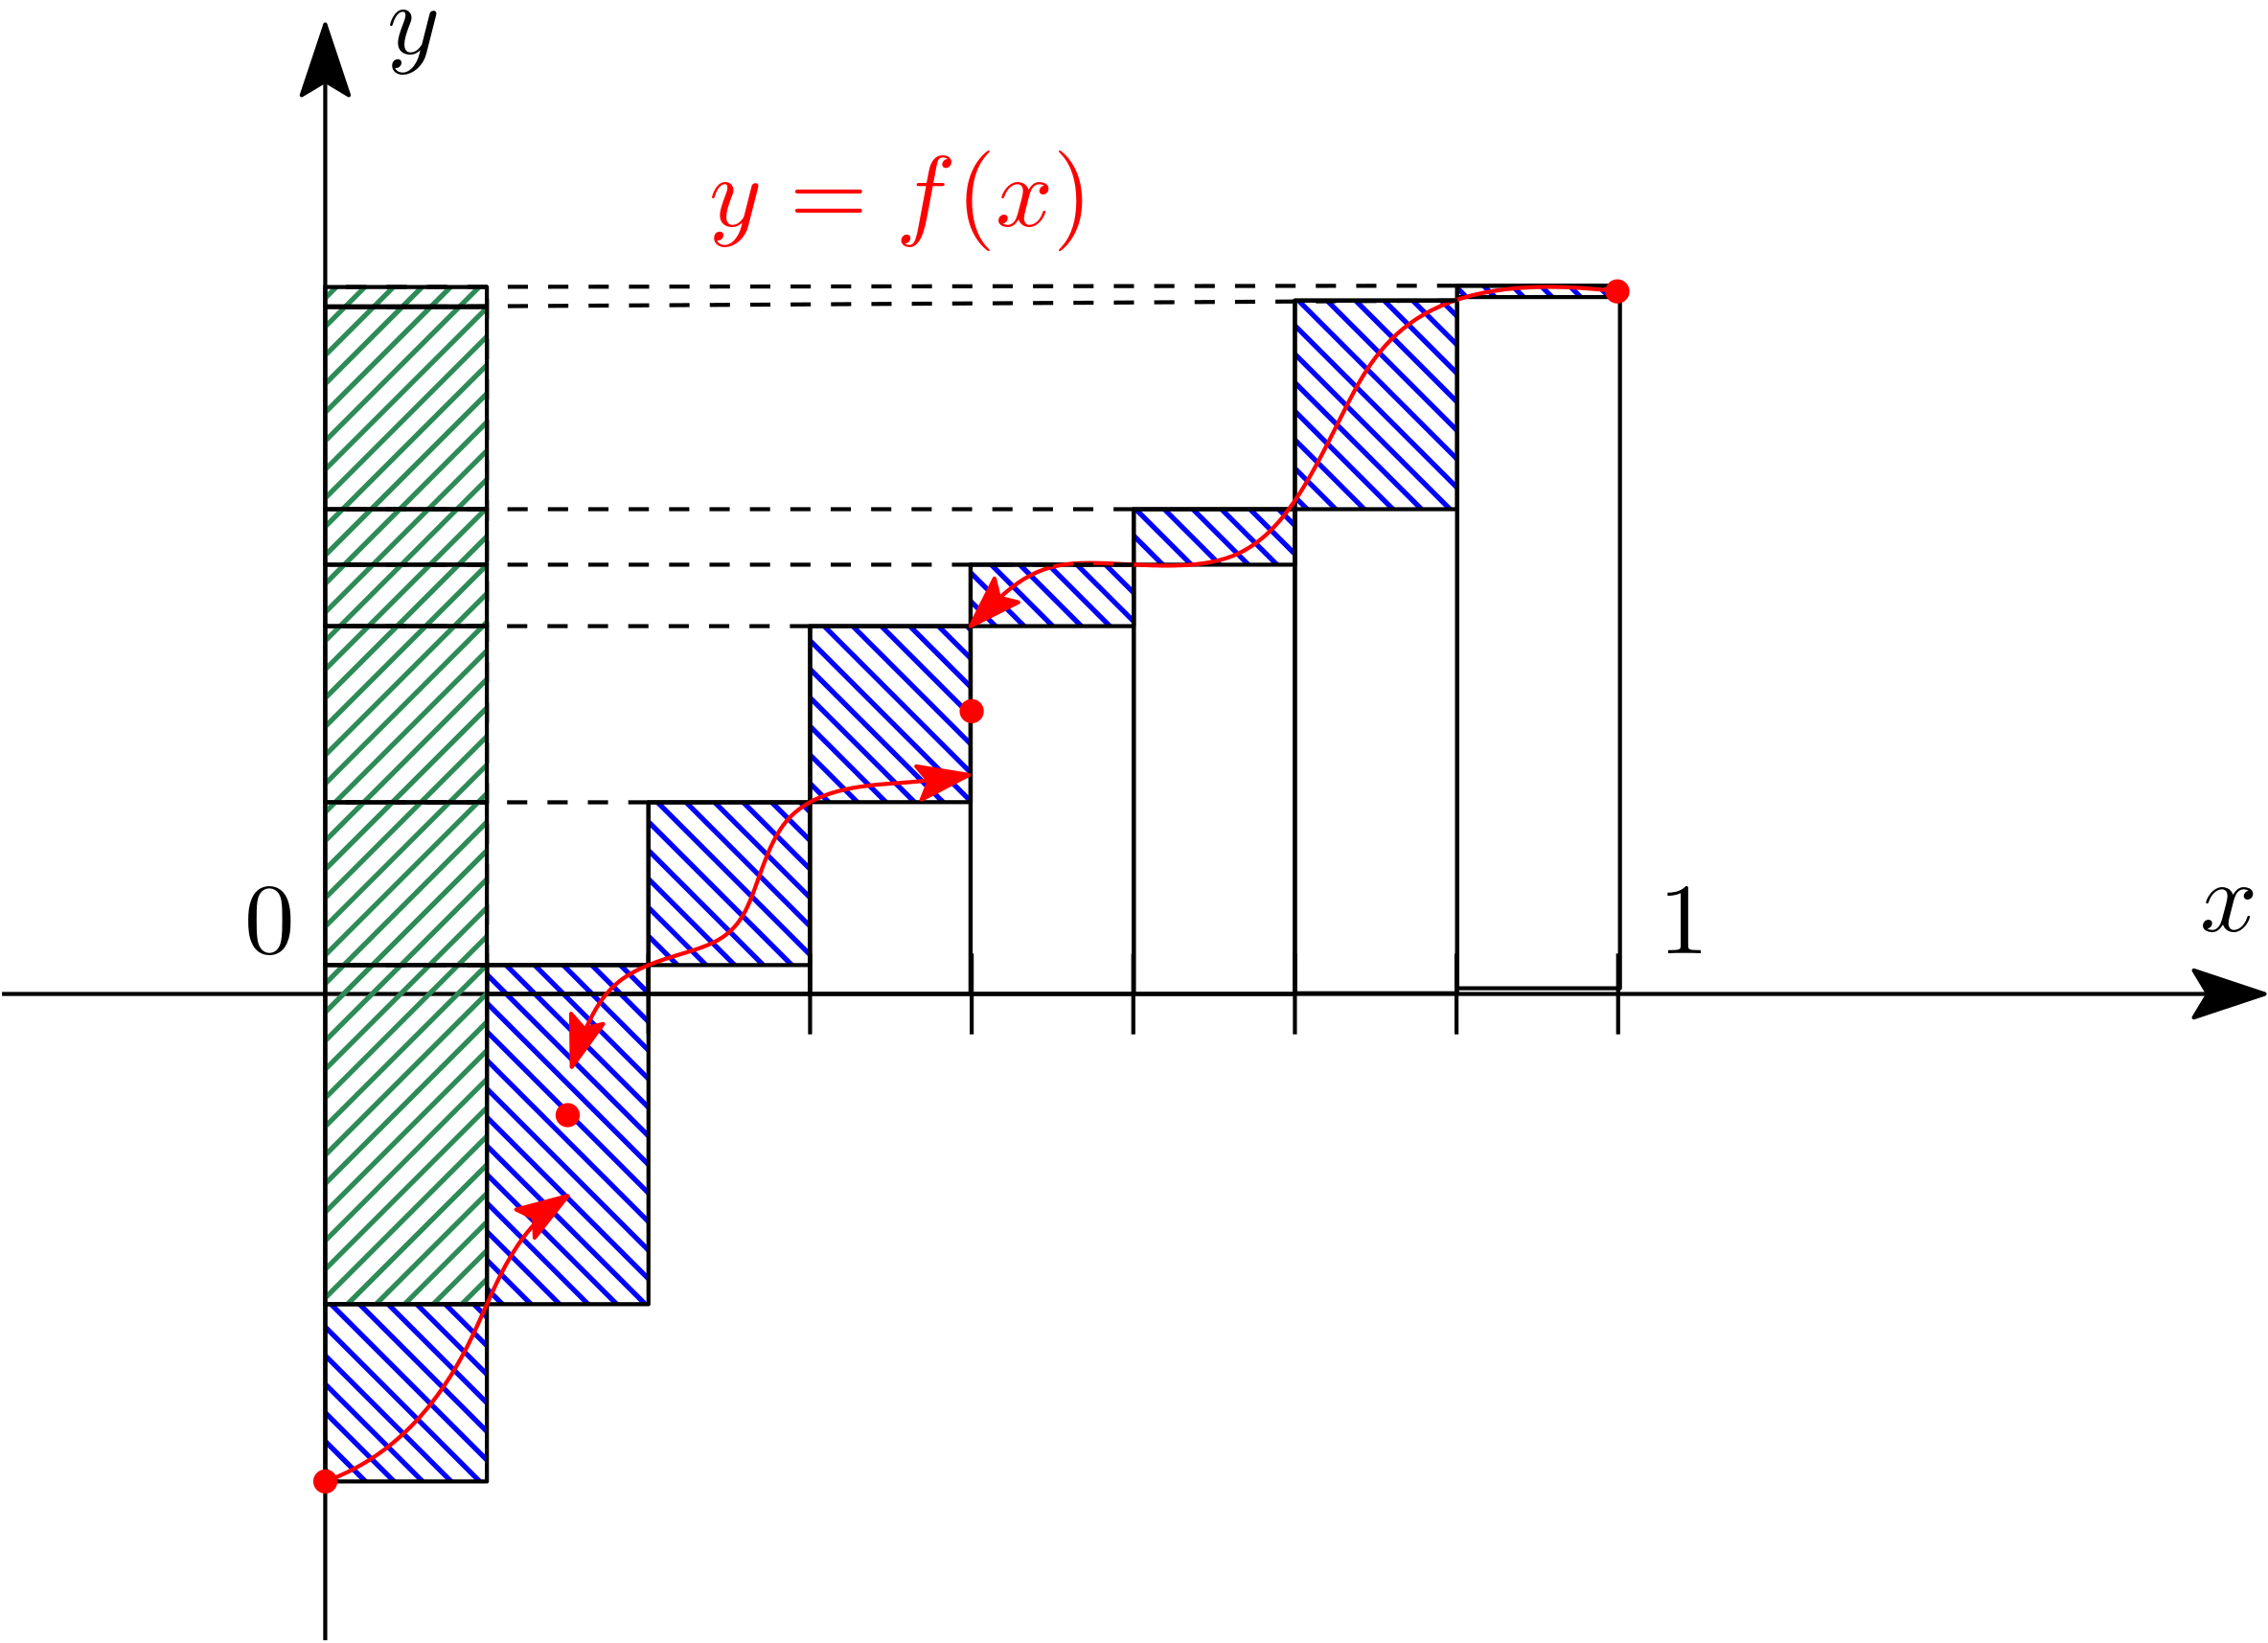
\includegraphics[width=0.45\textwidth]{MA2S8_6.png}
		\caption{Суммы Дарбу для $f(x)$, разность между ними (зазор между суммами) и перенесенная разность.}
		\label{8_6}
	\end{figure}
	Перенесем эти разности параллелльно в крайний левый прямоугольник. Все такие перенесенные части не будут пересекать друг друга (только по верхним и нижним краям). Площадь полученного прямоугольника будет равна:
	$$
		S(f,\MTB) - s(f,\MTB) = (f(1) - f(0)){\cdot}\dfrac{1}{n}
	$$
	Отсюда мы видим, что интеграл существует, поскольку нижняя и верхняя суммы сколь угодно близко приближаются друг к другу. Заметим, что поскольку $s(f,\MTB) \leq \sigma(f,\MTB,\xi) \leq S(f,\MTB)$, то:
	$$
		|\MI - S(f,\MTB)| \leq S(f,\MTB) - s(f,\MTB) = (f(1) - f(0)){\cdot}\dfrac{1}{n}
	$$
	$$
		0\leq n{\cdot}|\MI - S(f,\MTB)|\leq f(1) - f(0) \Rightarrow \text{ограниченная} \Rightarrow |\MI - S(f,\MTB)| = O\left(\dfrac{1}{n}\right)
	$$
\end{proof}
\begin{rem}
	К примеру, если попросят посчитать интеграл от монотонной функции и мы посчитаем его с точностью до $0,01$, то мы смотрим насколько функция меняется: $f(1) - f(0)$ и подбираем $n$ так, чтобы:
	$$
		\dfrac{f(1) - f(0)}{n} \leq \dfrac{1}{100}
	$$
\end{rem}
\section*{Формула Ньютона-Лейбница}

\begin{theorem}(\textbf{формула Ньютона-Лейбница})
	Если $f(x)$ - непрерывна, то у неё есть первообразная такая, что:
	$$
		\ddint{a}{b}f(x)dx = F(b) - F(a), \quad F'(x) \equiv f(x)
	$$
	Можно немного ослабить условие, тогда будет существовать обобщенная первообразная, то есть существует конечное множество $E$ такое, что $\forall x \in [a,b]\setminus E$ верно:
	$$
		F'(x) \equiv f(x), \, F(x) \in C[a,b]
	$$
\end{theorem}

\textbf{Пример когда формула не работает}: у лестница Кантора $F'(x)$ существует всюду за исключением точек множества Кантора и производная $F'(x) = 0$, поскольку эта функция на любом интервале вне точек множества Кантора постоянная и растёт только в этих точках. $F'(x)$ существует всюда за исключением точек множества Кантора. Функция при этом будет непрерывной, но тем не менее:
$$
	\ddint{0}{1}0\, dx \neq 1 = F(1) - F(0) = 1 - 0
$$

\begin{problem}
	Проинтегрируем функцию из задачи \textbf{Д2182 а)}:
	$$
		\ddint{-2}{3}x^3dx
	$$
\end{problem}
\begin{proof}
	$$
		\ddint{-2}{3}x^3dx = \dfrac{x^4}{4}\bigg|_{x = -2}^{3} = \dfrac{81 - 16}{4} = \dfrac{65}{4}
	$$
\end{proof}

Отметим, что формула Ньютона-Лейбница не всегда нормально работает. Для этого рассмотрим следующую задачу.
\begin{problem}(\textbf{Д2216 а)})
	$$
		\ddint{-1}{1}\dfrac{dx}{x}
	$$
\end{problem}
\begin{proof}
	Сначала рассмотрим неправильное решение:
	$$
		\ddint{-1}{1}\dfrac{dx}{x} = \ln{|x|}\bigg|_{x = -1}^{1} = 0
	$$
	Это не так, потому что надо проверять условия формулы Ньютона-Лейбница. Помимо того, что у логарифма производная есть всюду за исключением точки $0$, необходимо чтобы $F(x) \in C[-1,1]$, а она разрывна в $0$ и как-то склеить её, доопределить, до непрерывной не получится. Более того, $\tfrac{1}{x}$ - не ограничена $\Rightarrow$ интеграла Римана не существует.
\end{proof}

\begin{problem}(\textbf{Д2216 б)})
	Найти значение:
	$$
		\ddint{0}{2\pi}\dfrac{\tfrac{1}{\cos^2{x}}}{2 + \tg^2{x}}dx
	$$
\end{problem}
\begin{proof}
	Сначала рассмотрим неправильное решение, мы либо можем пользоваться формулой замены переменных, либо можем угадать первообразную. Рассмотрим первообразную функции:
	$$
		\dint \dfrac{1}{a + t^2} = \dfrac{1}{\sqrt{a}}\arctg{\left(\dfrac{t}{\sqrt{a}}\right)} + C \Rightarrow t = \tg{x} \Rightarrow \left(\dfrac{1}{\sqrt{2}}\arctg{\left(\dfrac{\tg{x}}{\sqrt{2}}\right)}\right)'  = \dfrac{\tfrac{1}{\cos^2{x}}}{2 + \tg^2{x}}
	$$
	Сделаем подстановку:
	$$
		\dfrac{1}{\sqrt{2}}\arctg{\left(\dfrac{\tg{x}}{\sqrt{2}}\right)}\bigg|_{x = 0}^{2\pi} = 0 - 0 = 0
	$$
	Смущает что подинтегральная функция - положительна, почему площадь подграфика положительной функции равна нулю? Например, $\tfrac{1}{\cos^2{x}}$ определён не везде, тогда рассмотрим функцию в виде:
	$$
		\dfrac{\tfrac{1}{\cos^2{x}}}{2 + \tg^2{x}} = \dfrac{1}{2\cos^2{x} + \sin^2{x}} > 0
	$$ 
	Полученная функция ограниченна и положительна, её производная будет совпадать с производной исходной функции и равна нулю. В чем подвох? Есть точки разрыва у $F(x)$. Рассмотрим их:
	$$
		x \to \dfrac{\pi}{2}- \Rightarrow \tg{x} \to +\infty \Rightarrow \dfrac{1}{\sqrt{2}}\arctg{\left(\dfrac{\tg{x}}{\sqrt{2}}\right)} \to \dfrac{\pi}{2\sqrt{2}}
	$$
	$$
		x \to \dfrac{\pi}{2}+ \Rightarrow  \tg{x} \to -\infty \Rightarrow \dfrac{1}{\sqrt{2}}\arctg{\left(\dfrac{\tg{x}}{\sqrt{2}}\right)} \to -\dfrac{\pi}{2\sqrt{2}}
	$$
	Поскольку арктангенс это $\pi$-периодическая функция, то аналогичная картина будет и для $\tfrac{3\pi}{2}$. Следовательно, функция не является непрерывной и формулу Ньютона-Лейбница к ней применить нельзя. 
	
	Но на интервале $\left(\tfrac{\pi}{2}, \tfrac{3\pi}{2}\right)$ мы можем прибавить $\tfrac{\pi}{\sqrt{2}} \Rightarrow$ это поднимет график функции арктангенса и склеит две точки $\Rightarrow$ предел слева и справа будут одинаковыми. Аналогично проделывая прибавление $\pi \sqrt{2}$ для второго интервала $\left(\tfrac{3\pi}{2},2\pi \right)$ мы также получим подъем функции и равенство пределов слева и справа. И таким образом, первообразная будет иметь вид:
	$$
		F(x) = 
		\begin{cases}
			\tfrac{1}{\sqrt{2}}\arctg{\left(\tfrac{\tg{x}}{\sqrt{2}}\right)}, & x \in \left[0, \tfrac{\pi}{2}\right) \\
			\tfrac{1}{\sqrt{2}}\arctg{\left(\tfrac{\tg{x}}{\sqrt{2}}\right)} + \dfrac{\pi}{\sqrt{2}},  & x \in \left(\tfrac{\pi}{2},\tfrac{3\pi}{2}\right)\\
	 		\tfrac{1}{\sqrt{2}}\arctg{\left(\tfrac{\tg{x}}{\sqrt{2}}\right)} + \pi\sqrt{2}, & x \in \left(\tfrac{3\pi}{2},2\pi\right]\\[10pt]
	 		\dfrac{\pi}{2\sqrt{2}}, & x = \tfrac{\pi}{2}\\[10pt]
	 		\pi\sqrt{2}, & x = \tfrac{3\pi}{2}
	 		
		\end{cases}
	$$
	таким образом, мы получили функцию, которая является обобщенной первообразной. Следовательно:
	$$
		\ddint{0}{2\pi}\dfrac{\tfrac{1}{\cos^2{x}}}{2 + \tg^2{x}}dx = F(2\pi) - F(0) = \sqrt{2}\pi - 0 = \sqrt{2}\pi
	$$
\end{proof}

\textbf{ДЗ}: $2182$ б), $2189$ с подсказкой, $2192^*$ - необязательная и трудная, $2193.2$ (картинкой решается легко), $2200$, $2205$, $2207$, $2209$, $2216$ в).

\end{document}